\chapter{Sequence Modelling}
\section{Introduction}
Sequence Modelling is the ability of a computer program to model, interpret, make predictions about or generate any type of sequential data, such as audio, text etc. For example, a computer program that can take a piece of text in English and translate it to French is an example of a Sequence Modelling program (because the type of data being dealt with is text, which is sequential in nature). An AI algorithm called the Recurrent Neural Network, is a specialised form of the classic Artificial Neural Network (Multi-Layer Perceptron) that is used to solve Sequence Modelling problems. Recurrent Neural Networks are like Artificial Neural Networks which has loops in them. This means that the activation of each neuron or cell depends not only on the current input to it but also its previous activation values.

\section{Recurrent Neural Networks}
Humans don\textquotesingle t start their thinking from scratch every second. As we read a text, we understand each word based on your understanding of previous words. We don\textquotesingle t throw everything away and start thinking from scratch again. Our thoughts have persistence.

Traditional neural networks can\textquotesingle t do this, and it seems like a major shortcoming. For example, imagine you want to classify what kind of event is happening at every point in a movie. It\textquotesingle s unclear how a traditional neural network could use its reasoning about previous events in the film to inform later ones.

Recurrent neural networks address this issue. They are networks with loops in them, allowing information to persist.

\begin{figure}[H]
    \centering
    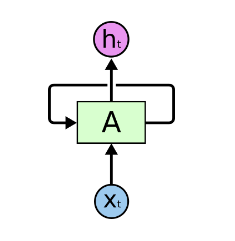
\includegraphics[scale = 0.9]{rnn.png}
    \caption{Recurrent Neural Networks}
    \label{fig:RNNs}
\end{figure}

In the above diagram, a chunk of neural network, A, looks at some input xt and outputs a value ht. A loop allows information to be passed from one step of the network to the next.

These loops make recurrent neural networks seem kind of mysterious. However, if you think a bit more, it turns out that they aren\textquotesingle t all that different than a normal neural network. A recurrent neural network can be thought of as multiple copies of the same network, each passing a message to a successor. Consider what happens if we unroll the loop:

\begin{figure}[H]
    \centering
    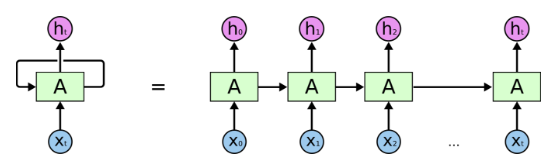
\includegraphics[scale = 0.8]{Unfolded_rnn.png}
    \caption{An unrolled recurrent neural networks}
    \label{fig:Unrolled RNNs}
\end{figure}

This chain-like nature reveals that recurrent neural networks are intimately related to sequences and lists. They\textquotesingle re the natural architecture of neural network to use for such data.

And they certainly are used! In the last few years, there have been incredible success applying RNNs to a variety of problems: speech recognition, language modeling, translation, image captioning, etc.

\section{Vanishing Gradients with RNNs}
One of the appeals of RNNs is the idea that they might be able to connect previous information to the present task, such as using previous video frames might inform the understanding of the present frame. If RNNs could do this, they\textquotesingle d be extremely useful. But can they? It depends.

Sometimes, we only need to look at recent information to perform the present task. For example, consider a language model trying to predict the next word based on the previous ones. If we are trying to predict the last word in “the clouds are in the sky,” we don\textquotesingle t need any further context - it\textquotesingle s pretty obvious the next word is going to be sky. In such cases, where the gap between the relevant information and the place that it\textquotesingle s needed is small, RNNs can learn to use the past information.

\begin{figure}[H]
    \centering
    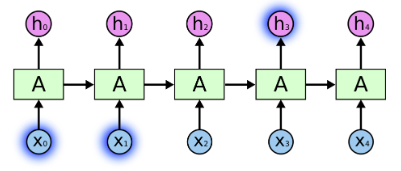
\includegraphics[scale = 0.8]{Short Sequence in RNNs.png}
    \caption{Short Sequence in RNNs}
    \label{fig:Short seq in  RNNs}
\end{figure}

But there are also cases where we need more context. Consider trying to predict the last word in the text “I grew up in France… I speak fluent French.” Recent information suggests that the next word is probably the name of a language, but if we want to narrow down which language, we need the context of France, from further back. It\textquotesingle s entirely possible for the gap between the relevant information and the point where it is needed to become very large.

Unfortunately, as that gap grows, RNNs become unable to learn to connect the information.

\begin{figure}[H]
    \centering
    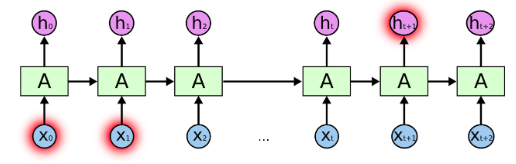
\includegraphics[scale = 0.8]{Long Sequence in RNNs.png}
    \caption{Long Sequence in RNNs}
    \label{fig:Short Sequence in RNNs}
\end{figure}

In theory, RNNs are absolutely capable of handling such “long-term dependencies.” A human could carefully pick parameters for them to solve toy problems of this form. Sadly, in practice, RNNs don\textquotesingle t seem to be able to learn them. The problem was explored in depth by Hochreiter (1991) [German] and Bengio, et al. (1994), who found some pretty fundamental reasons why it might be difficult.


\section{LSTMs}
Long Short Term Memory networks - usually just called “LSTMs” - are a special kind of RNN, capable of learning long-term dependencies. They were introduced by Hochreiter and Schmidhuber (1997), and were refined and popularized by many people in following work. They work tremendously well on a large variety of problems, and are now widely used.

LSTMs are explicitly designed to avoid the long-term dependency problem. Remembering information for long periods of time is practically their default behavior, not something they struggle to learn!

All recurrent neural networks have the form of a chain of repeating modules of neural network. In standard RNNs, this repeating module will have a very simple structure, such as a single tanh layer as shown below.

\begin{figure}[H]
    \centering
    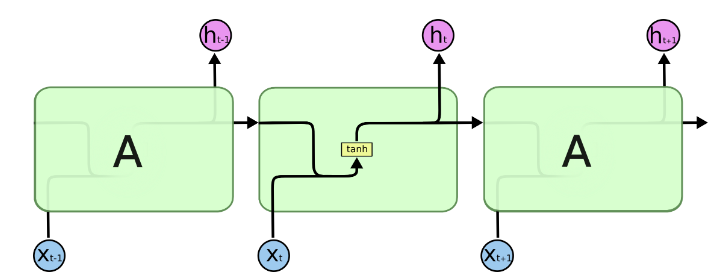
\includegraphics[scale = 0.65]{RNNs_repeating.png}
    \caption{The repeating module in a standard RNN contains a single layer.}
    \label{fig:RNNs_repeating}
\end{figure}

LSTMs also have this chain like structure, but the repeating module has a different structure. Instead of having a single neural network layer, there are four, interacting in a very special way.


\begin{figure}[H]
    \centering
    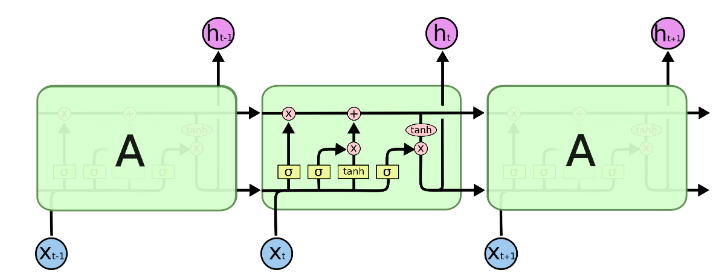
\includegraphics[scale = 0.65]{LSTMs_repeating.png}
    \caption{The repeating module in an LSTM contains four interacting layers.}
    \label{fig:LSTMs_repeating}
\end{figure}

\subsection{LSTM Cell}
The following figure shows the operations of an LSTM cell:
\begin{figure}[H]
    \centering
    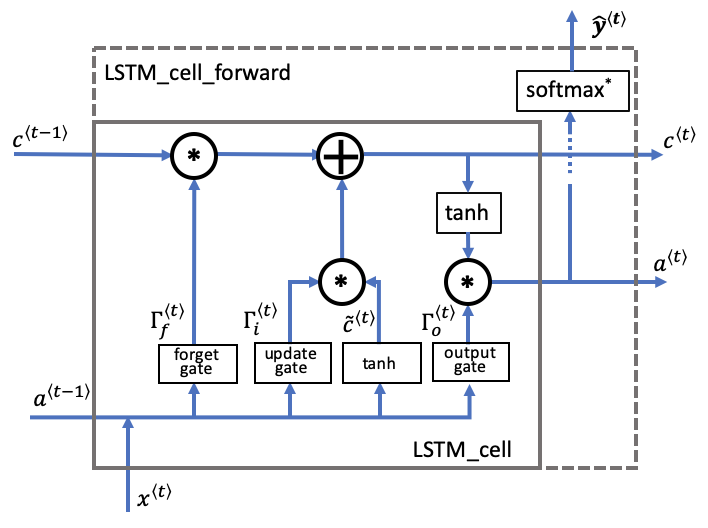
\includegraphics[scale = 1]{LSTM_cell.png}
    \caption{LSTM Cell}
    \label{fig:LSTMs_cell}
\end{figure}

\subsubsection{Forget Gate $\Gamma _f$}
Assume, we are reading words in a piece of text and plan to use an LSTM to keep track of grammatical structures, such as whether the subject is singular("dog") or plural("dogs). If the subject changes its state (from a singular word to a plural word), the memory of the previous state becomes outdated, so it is better to forget that outdated state.

The forget gate is a tensor containing values between 0 and 1. If a unit in the forget gate has a value close to 0, the LSTM will forget the stored state in the corresponding unit of the previous cell state. If a unit in the forget gate has a value close to 1, the LSTM will mostly remember the corresponding value in the stored state.

\begin{equation}
    \Gamma _f ^{<t>} = \sigma (W_f[a^{<t - 1>}, x^{<t>}] + b_f)
\end{equation}

where,
\begin{itemize}
    \item $W_f$ = forget gate weight $W_f$
    \item $b_f$ = forget gate bias $b_f$
    \item $\Gamma _f ^ {<t>}$ = Forget Gate
\end{itemize}

Explanation of the equation:
\begin{itemize}
    \item $W_f$ contains the weights that govern the forget gate\textquotesingle s behavior.
    \item The previous time step's hidden state $a^{<t - 1>}$  and current time step's input $x^{<t>}$ are concatenated together and multiplied by $W_f$.
    \item A sigmoid function is used to make each of the gate tensor's values $\Gamma _f ^ {<t>}$ range from 0 to 1.
    \item The forget gate $\Gamma _f ^ {<t>}$
          has the same dimensions as the previous cell state $c^{<t - 1>}$.
    \item Multiplying the tensors $\Gamma _f ^ {<t>}$ * $c^{<t - 1>}$
          is like applying a mask over the previous cell state.
    \item If a single value in $\Gamma _f ^ {<t>}$ is 0 or close to 0, then the product is close to 0. This keeps the information stored in the corresponding unit in $c^{<t - 1>}$ from being remembered for the next time step.
    \item Similarly, if one value is close to 1, the product is close to the original value in the previous cell state. The LSTM will keep the information from the corresponding unit of $c^{<t - 1>}$, to be used in the next time step.
\end{itemize}

\subsubsection{Candidate Value $\tilde{c}^{<t>}$}
The candidate value is a tensor containing information from the current time step that may be stored in the current cell state $c^{<t>}$. The parts of the candidate value that get passed on depend on the update gate.
The candidate value is a tensor containing values that range from -1 to 1.
The tilde "~" is used to differentiate the candidate $\tilde{c}^{<t>}$ from the cell state $c^{<t>}$.

\begin{equation}
    \tilde{c}^{<t>} = tanh(W_c[a^{<t - 1>}, x^{<t>}] + b_c)
\end{equation}

\subsubsection{Update Gate $\Gamma _i$}
Update gate can be used to decide what aspects of the candidate $\tilde{c}^{<t>}$ to add to the cell state $c^{<t>}$. The update gate is a tensor containing values between 0 and 1. When a unit in the update gate is close to 1, it allows the value of the candidate $\tilde{c}^{<t>}$ to be passed onto the hidden state $c^{<t>}$. When a unit in the update gate is close to 0, it prevents the corresponding value in the candidate from being passed onto the hidden state.

\begin{equation}
    \Gamma _i ^ {<t>} = \sigma (W_i[a^{<t - 1>}, x^{<t>}] + b_i)
\end{equation}

Explanation of the equation:
\begin{itemize}
    \item Similar to the forget gate, here $\Gamma _i ^{<t>}$
          , the sigmoid produces values between 0 and 1.
    \item The update gate is multiplied element-wise with the candidate, and this product $\Gamma _i ^{<t>}$ * $\tilde{c}^{<t>}$ is used in determining the cell state $c^{<t>}$.
\end{itemize}

\subsubsection{Cell State $c^{<t>}$}
The cell state is the "memory" that gets passed onto future time steps.
The new cell state $c^{<t>}$ is a combination of the previous cell state and the candidate value.

\begin{equation}
    c^{<t>} = \Gamma _f ^{<t>} * c^{<t - 1>} + \Gamma _i ^{<t>} * \tilde{c}^{<t>}
\end{equation}

Explanation of the equation
\begin{itemize}
    \item The previous cell state $c^{<t - 1>}$
          is adjusted (weighted) by the forget gate $\Gamma _f ^{<t>}$.
    \item the candidate value $\tilde{c}^{<t>}$ is adjusted (weighted) by the update gate $\Gamma _i ^{<t>}$.
\end{itemize}

\subsubsection{Output Gate $\Gamma _o$}
The output gate decides what gets sent as the prediction (output) of the time step. The output gate is like the other gates, in that it contains values that range from 0 to 1.

\begin{equation}
    \Gamma _o ^ {<t>} = \sigma (W_o[a^{<t - 1>}, x^{<t>}] + b_o)
\end{equation}

Explanation of the equation
\begin{itemize}
    \item The output gate is determined by the previous hidden state $a^{<t - 1>}$ and the current input $x^{t}$
    \item The sigmoid makes the gate range from 0 to 1.
\end{itemize}

\subsubsection{Hidden State $a^{<t>}$}
The hidden state gets passed to the LSTM cell's next time step. It is used to determine the three gates ($\Gamma _f , \Gamma _u , \Gamma _o $) of the next time step. The hidden state is also used for the prediction $y^{<t>}$.

\begin{equation}
    a^{<t>} = \Gamma _o ^{<t>} * tanh(c^{<t>})
\end{equation}

Explanation of the equation
\begin{itemize}
    \item The hidden state $a^{<t>}$
          is determined by the cell state $c^{<t>}$
          in combination with the output gate $\Gamma _o$.
    \item The cell state state is passed through the tanh function to rescale values between -1 and 1.
    \item The output gate acts like a "mask" that either preserves the values of tanh($c^{<t>}$) or keep those values from being included in the hidden state $a^{<t>}$.
\end{itemize}

\subsubsection{Prediction $y_{pred}^{<t>}$}
The prediction in this use case is a classification, so you'll use a softmax.

\begin{equation}
    y_{pred}^{<t>} = softmax(W_y a^{<t>} + b_y)
\end{equation}

\section{Bidirectional RNNs}
A typical state in an RNN (simple RNN, GRU, or LSTM) relies on the past and the present events. A state at time t depends on the states $x_1$, $x_2$, ...., $x_{t - 1}$ and $x_{t}$. However, there can be situations where a prediction depends on the past, present, and future events.

For example, predicting a word to be included in a sentence might require us to look into the future, i.e., a word in a sentence could depend on a future event. Such linguistic dependencies are customary in several text prediction tasks.  

Thus, capturing and analyzing both past and future events is helpful in the above-mentioned scenarios.

To enable straight (past) and reverse traversal of input (future), Bidirectional RNNs, or BRNNs, are used. A BRNN is a combination of two RNNs - one RNN moves forward, beginning from the start of the data sequence, and the other, moves backward, beginning from the end of the data sequence. The network blocks in a BRNN can either be simple RNNs, GRUs, or LSTMs.

\begin{figure}[H]
    \centering
    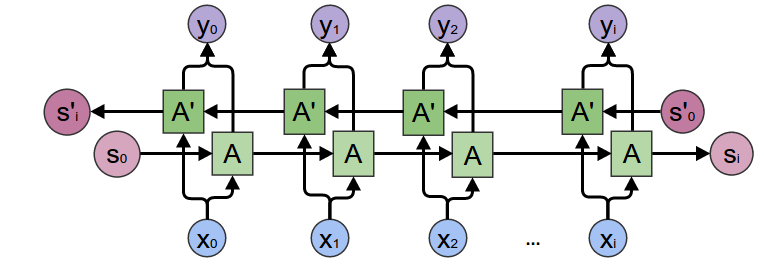
\includegraphics[scale = 0.6]{BRNNs.png}
    \caption{Bidirectional RNN}
    \label{fig:BRNN}
\end{figure}

\section{Sequence Modelling Applications}
Some applications of sequence modelling are:
\begin{itemize}
    \item \textbf{Language Modelling} : Auto-generation of next probable word.(Previous sequence of words are sequential data)
    \item \textbf{Image Captioning} (with the help of computer vision): Generating captions for images. (captions are sequential data)
    \item \textbf{Video Frame Prediction} (with the help of computer vision): Predict the subsequent frames of video given the previous ones. (the frames in a video are sequential in nature)
    \item \textbf{Classifying songs} (audio) as Jazz, Rock , Pop etc (genre). Here, audio is of sequential nature.
    \item \textbf{Composing Music} (music is sequential in nature)
\end{itemize}


